\section{Basic Functionalities guide}
\subsection{Functional Elements}

\subsubsection{ExternalAPI}
ExternalAPI is a useful element capable of retrieving a \glossario{JSON} file from an \glossario{API} method and storing it in the Bubble. 
\begin{figure}[H]
 	\centering
 	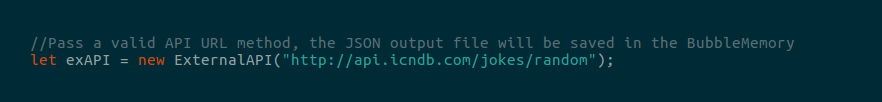
\includegraphics[width=14cm]{../../documenti/UserManualFramework/framework_model/1framework_model_api.png}
 	\caption{ExternalAPI}
\end{figure}

\subsubsection{WebNotification}
Through WebNotification it is possible to show the user a notification, to create the notification a user has to specify a title, an icon and some text. 
\begin{figure}[H]
	\centering
	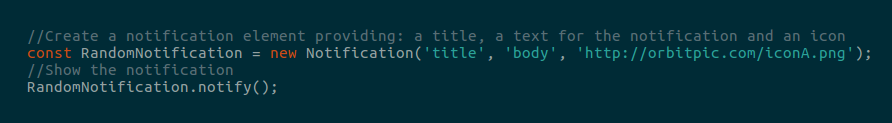
\includegraphics[width=14cm]{../../documenti/UserManualFramework/framework_model/2framework_model_notification.png}
	\caption{WebNotification}
\end{figure}

\subsubsection{Database}
The functional element Database is based on the \glossario{MongoDB} collection system, it is used to write and read data in the collections by simply specifying an URL pointing to a MongoDB instance and the name of a collection.
\begin{figure}[H]
	\centering
	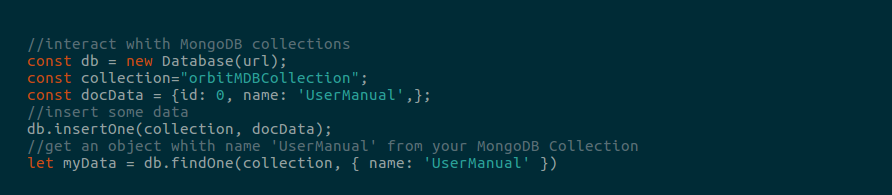
\includegraphics[width=14cm]{../../documenti/UserManualFramework/framework_model/3framework_model_mongo.png}
	\caption{MongoDB}
\end{figure}

\subsubsection{MatchRegularExpr}
MatchRegularExpr stores a regular expression and allows the user to execute different methods of MatchRegularExpr on some text.
It can either operate in \glossario{Case Sensitive} Mode or Multi-line mode and can execute multiple matches for a given text.
MatchRegularExpr can combine strings and regexp to create other MatchRegularExpr objects.
\begin{figure}[H]
	\centering
	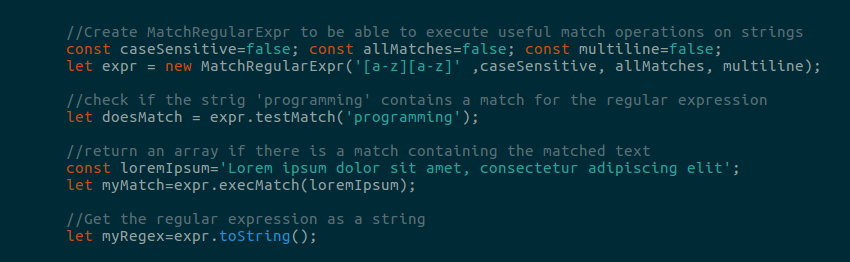
\includegraphics[width=14cm]{../../documenti/UserManualFramework/framework_model/5framework_model_regexp1.png}
	\caption{MatchRegularExpr}
\end{figure}

\begin{figure}[H]
	\centering
	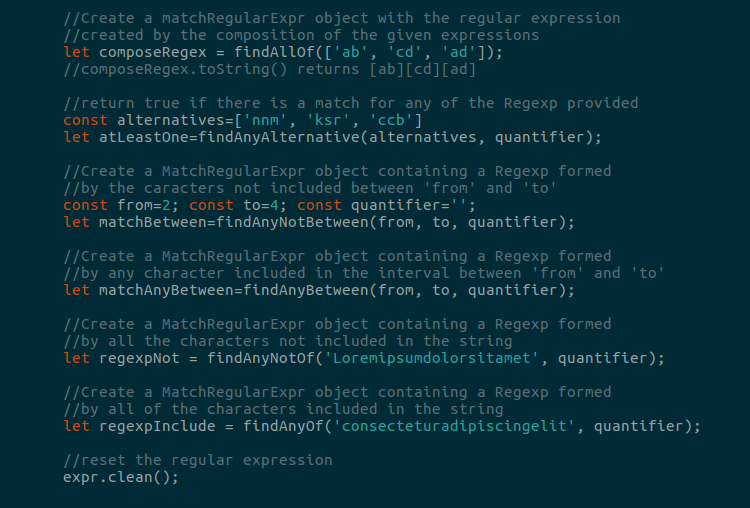
\includegraphics[width=14cm]{../../documenti/UserManualFramework/framework_model/6framework_model_regexp2.png}
	\caption{Regular Expressions}
\end{figure}

\subsubsection{Action}
An action is executed on an object, is is described by a string, in the following example we are creating a DELETE action. 
\begin{figure}[H]
	\centering
	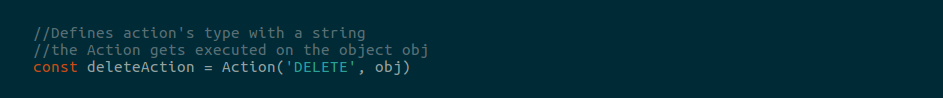
\includegraphics[width=14cm]{../../documenti/UserManualFramework/framework_model/Action.png}
	\caption{Action}
\end{figure}

\subsubsection{IDGenerator}
IDGenerator generates random id objects for a MongoDB DataBase. It is possible to get a String version of the id.
\begin{figure}[H]
	\centering
	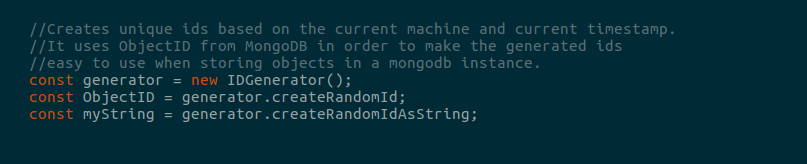
\includegraphics[width=14cm]{../../documenti/UserManualFramework/framework_model/idGenerator.png}
	\caption{IDGenerator}
\end{figure}

\subsubsection{Server}
Server istantiate an ExpressApp.
\begin{figure}[H]
	\centering
	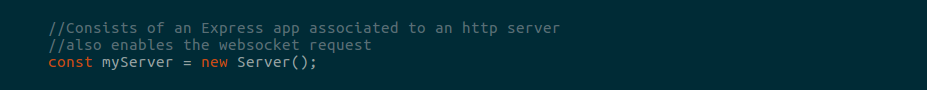
\includegraphics[width=14cm]{../../documenti/UserManualFramework/framework_model/Server.png}
	\caption{Server}
\end{figure}

\subsubsection{User}
A User consists of a username and a role. It is possible to get the username of a User.
\begin{figure}[H]
	\centering
	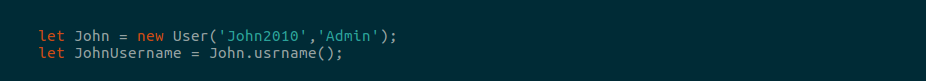
\includegraphics[width=14cm]{../../documenti/UserManualFramework/framework_model/User.png}
	\caption{User}
\end{figure}

\subsection{Graphical Elements}\label{GraphicalElements}
\subsubsection{Button}
In a Button tag it is possible to specify the text for the button and to bind a function that will be called when the button is clicked.
\begin{figure}[H]
	\centering
	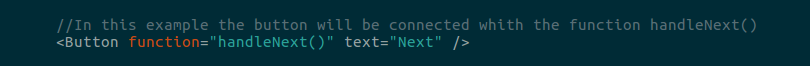
\includegraphics[width=14cm]{../../documenti/UserManualFramework/framework_view/11framework_view_button.png}
	\caption{Button}
\end{figure}

\begin{figure}[H]
	\centering
	
\includegraphics[width=6cm]{../../documenti/UserManualFramework/graphical_elements/buttonGE.png}
	\caption{Rendering of the Button}
\end{figure}

\subsubsection{Label}
A Label can be associated to an \glossario{HTML} element, it can contain some informative text regarding the element.
\begin{figure}[H]
	\centering
	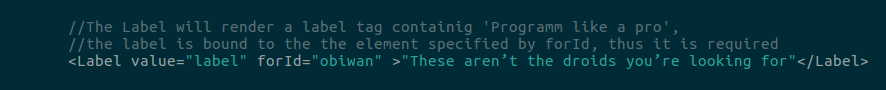
\includegraphics[width=14cm]{../../documenti/UserManualFramework/framework_view/12framework_view_label.png}
	\caption{Label}
\end{figure}

\begin{figure}[H]
	\centering
	
\includegraphics[width=6cm]{../../documenti/UserManualFramework/graphical_elements/labelGE.png}
	\caption{A Label associated to a CheckBox}
\end{figure}

\subsubsection{Image}
Image renders an image file and contains a caption describing that image.
\begin{figure}[H]
	\centering
	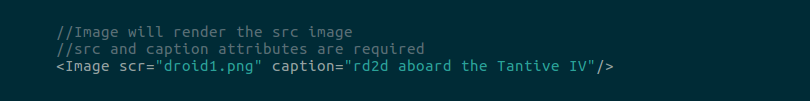
\includegraphics[width=14cm]{../../documenti/UserManualFramework/framework_view/13framework_view_image.png}
	\caption{Image}
\end{figure}

\subsubsection{TextView}
A TextView is a container for some text.
\begin{figure}[H]
	\centering
	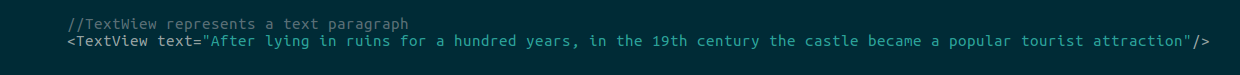
\includegraphics[width=14cm]{../../documenti/UserManualFramework/framework_view/14framework_view_textview.png}
	\caption{TextView}
\end{figure}

\begin{figure}[H]
	\centering
	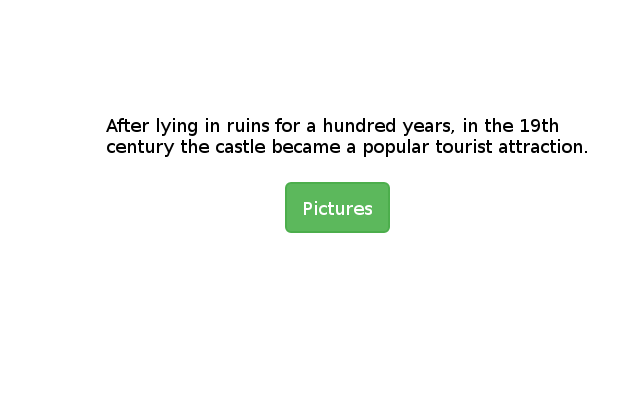
\includegraphics[width=10cm]{../../documenti/UserManualFramework/graphical_elements/textViewGE.png}
	\caption{TextView}
\end{figure}

\subsubsection{TextEdit}
A TextEdit contains a text paragraph and allows the user to interact with it, it is possble to bind a function to handle the editing.
\begin{figure}[H]
	\centering
	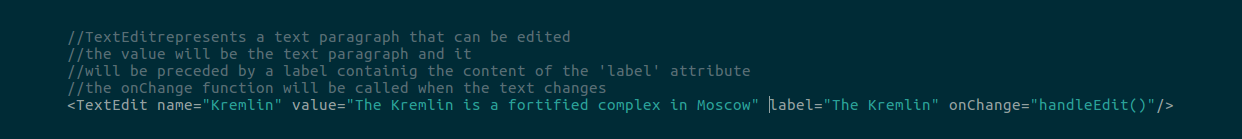
\includegraphics[width=14cm]{../../documenti/UserManualFramework/framework_view/15framework_view_textedit.png}
	\caption{TextEdit}
\end{figure}

\begin{figure}[H]
	\centering
	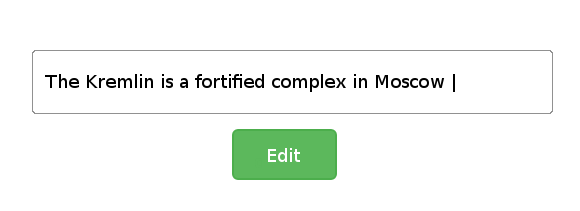
\includegraphics[width=10cm]{../../documenti/UserManualFramework/graphical_elements/textEditGE.png}
	\caption{TextEdit}
\end{figure}

\subsubsection{InputText}
InputText renders an input field for strings.
\begin{figure}[H]
	\centering
	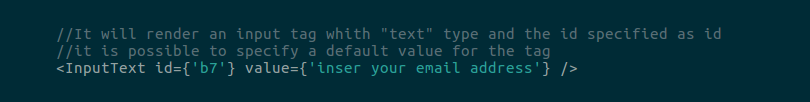
\includegraphics[width=14cm]{../../documenti/UserManualFramework/framework_view/16framework_view_inputtext.png}
	\caption{InputText}
\end{figure}

\begin{figure}[H]
	\centering
	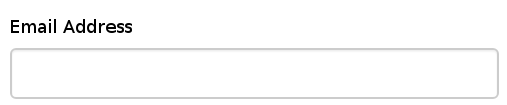
\includegraphics[width=6cm]{../../documenti/UserManualFramework/graphical_elements/inputTextGE.png}
	\caption{InputText}
\end{figure}

\subsubsection{InputFile}
InputText renders an input field for a file.
\begin{figure}[H]
	\centering
	
\includegraphics[width=14cm]{../../documenti/UserManualFramework/framework_view/17framework_view_inputfile.png}
	\caption{InputFile}
\end{figure}

\begin{figure}[H]
	\centering
	
\includegraphics[width=6cm]{../../documenti/UserManualFramework/graphical_elements/inputFileGE.png}
	\caption{InputFile}
\end{figure}

\subsubsection{RadioButton}
RadioButton represents a single instance of a button that will be placed together with other RadioButtons either in a RadioButtonGroup or in a simple sequence of RadioButtons.
\begin{figure}[H]
	\centering
	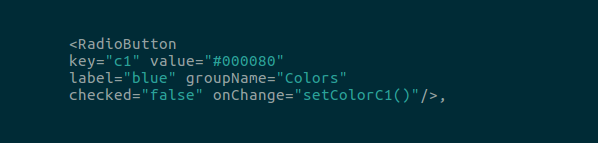
\includegraphics[width=14cm]{../../documenti/UserManualFramework/framework_view/7framework_view_radio.png}
	\caption{RadioButton}
\end{figure}

\subsubsection{RadioButtonGroup}
RadioButtonGroup represents a collection of RadioButtons.
RadioButtonGroup will require the user of the GUI to select a single RadioButton in the collection.
\begin{figure}[H]
	\centering
	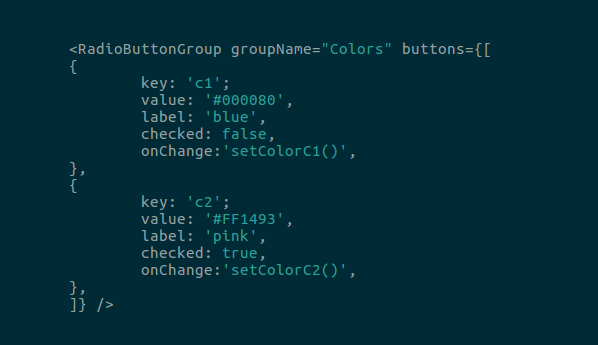
\includegraphics[width=14cm]{../../documenti/UserManualFramework/framework_view/8framework_view_radio_group.png}
	\caption{RadioButtonGroup}
\end{figure}

\begin{figure}[H]
	\centering
	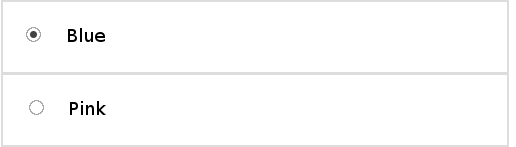
\includegraphics[width=6cm]{../../documenti/UserManualFramework/graphical_elements/radioButtonGroupGE.png}
	\caption{RadioButtonGroup}
\end{figure}

\subsubsection{CheckBox}
CheckBox represents a single instance of a button that will be placed together with other checkBoxes either in a CheckBoxGroup or in a simple sequence of CheckBoxes.
\begin{figure}[H]
	\centering
	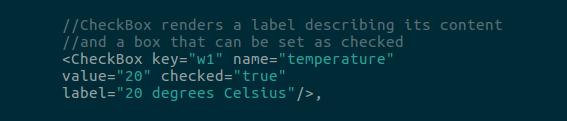
\includegraphics[width=14cm]{../../documenti/UserManualFramework/framework_view/9framework_view_check.png}
	\caption{checkBox}
\end{figure}

\subsubsection{CheckBoxGroup}
CheckBoxGroup represents a collection of CheckBoxes.
CheckBoxGroup will allow the user of the \glossario{GUI} to select any number of CheckBoxes.
\begin{figure}[H]
	\centering
	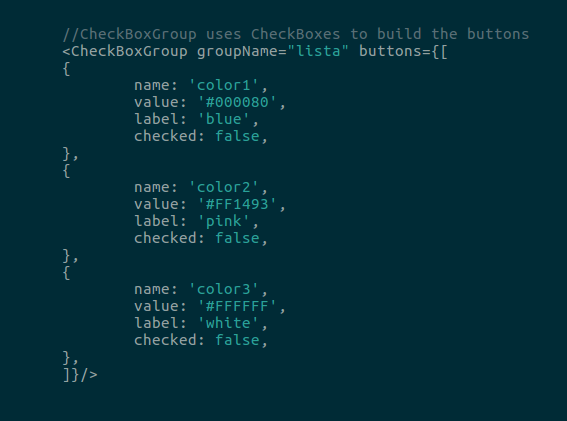
\includegraphics[width=14cm]{../../documenti/UserManualFramework/framework_view/10framework_view_check_group.png}
	\caption{CheckBoxGroup}
\end{figure}

\begin{figure}[H]
	\centering
	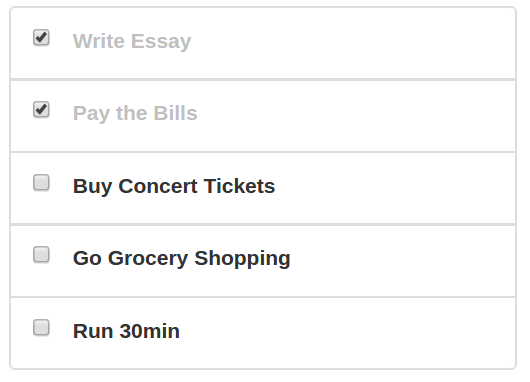
\includegraphics[width=6cm]{../../documenti/UserManualFramework/graphical_elements/checkBoxGroupGE.png}
	\caption{CheckBoxGroup}
\end{figure}

\subsubsection{BarChart}
BarChart allows to represent data whith bars that are proportional to the values they represent. It's possible to select colors for the bars and grid limits.
\begin{figure}[H]
	\centering
	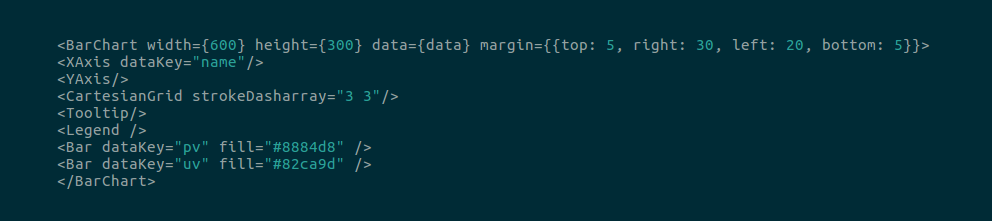
\includegraphics[width=14cm]{../../documenti/UserManualFramework/framework_view/18framework_view_bar.png}
	\caption{BarChart}
\end{figure}
\begin{figure}[H]
	\centering
	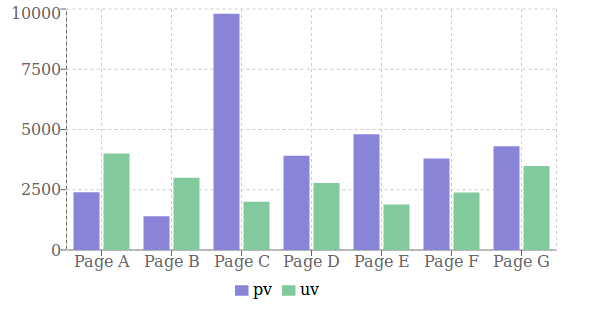
\includegraphics[width=14cm]{../../documenti/UserManualFramework/framework_view/barchart.png}
	\caption{BarChart example}
\end{figure}

\subsubsection{PieChart}
PieChart allows to represent data as a circle divided into slices. It's possible to specify the dimensions and colours for the pie chart. 
\begin{figure}[H]
	\centering
	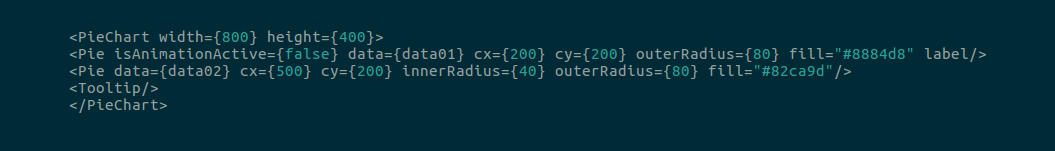
\includegraphics[width=14cm]{../../documenti/UserManualFramework/framework_view/19framework_view_pie.png}
	\caption{PieChart}
\end{figure}
\begin{figure}[H]
	\centering
	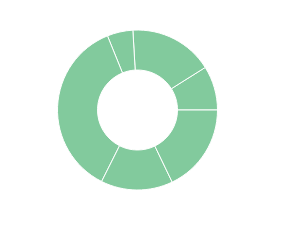
\includegraphics[width=14cm]{../../documenti/UserManualFramework/framework_view/piechart.png}
	\caption{PieChart example}
\end{figure}

\subsection{Bubbles}
\subsubsection{GenericBubble}
Import the GenericBubble class and place it inside your code to render your Generic Bubble. 
\begin{figure}[H]
	\centering
	
\includegraphics[width=14cm]{../../documenti/UserManualFramework/framework_view/20framework_view_generic.png}
	\caption{GenericBubble}
\end{figure}

\subsubsection{TodoBubble}
To render a To-do list import its class place it inside your code. 
\begin{figure}[H]
	\centering
	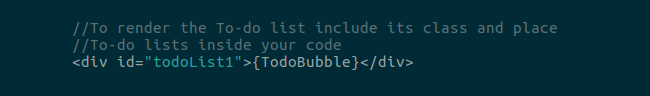
\includegraphics[width=14cm]{../../documenti/UserManualFramework/framework_view/22framework_view_todo.png}
	\caption{TodoBubble}
\end{figure}

\subsubsection{\DemoName{}}
\DemoName{} is built to support different types of users. To render a specific type of bubble import its class ad place the bubble inside your code.  
\begin{figure}[H]
	\centering
	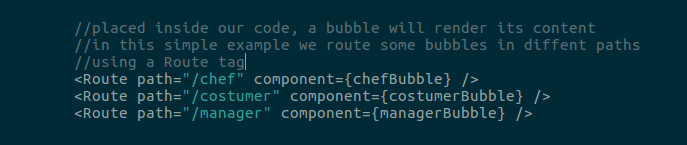
\includegraphics[width=14cm]{../../documenti/UserManualFramework/framework_view/21framework_view_demo.png}
	\caption{\DemoName{}}
\end{figure}
